\documentclass[aspectratio=169]{beamer}
\usetheme{AnnArbor}
\usecolortheme{beaver}
\usepackage[brazil]{babel} %texto
\usepackage[utf8]{inputenc} %texto
\usepackage{graphicx} %imagem	
\usepackage{caption} %imagem
\usepackage{subcaption} %imagem
\usepackage{float} %imagem e tabelas
\usepackage{booktabs} %tabelas	
\usepackage[abnt-emphasize=bf,alf]{abntex2cite} %citacoes ABNT
\usepackage{verbatim}
\graphicspath{{./Figuras/}} %Colarimages na pasta "Figuras". Gosto de fazer isso para organizar os arquivos.    		

%---------------------------------------------------------------------------
	% PRIMEIRA SECAO
	\section{Centro Federal de Educação Tecnológica de Minas Gerais}
	\subsection{Curso Técnico em Mecatrônica}
%---------------------------------------------------------------------------

\begin{document}
	% EDITAR ESSAS INFORMACOES (INICIO)
	\title[3º Relatório de Acompanhamento do Estagiário]{QUALIDADE E REPARO EM PROCESSOS INDUSTRIAIS DE GRANDE ESCALA}
	\subtitle{Aplicado a SmartPhones}
	\author[antonioaads@gmail.com]{Antônio Augusto Diniz Sousa}
	\institute[]{CEFET-MG}
	\date[2017]{\today}
	% EDITAR ESSAS INFORMACOES (FIM)
	
	\begin{frame}
		\titlepage
	\end{frame}
	\begin{frame}
		\frametitle{Sum\'{a}rio}
		\tableofcontents%[pausesections]
	\end{frame}
	
%---------------------------------------------------------------------------
	% PRIMEIRA SECAO
	\section{Global Express}
	\subsection{A empresa}
%---------------------------------------------------------------------------
	
	% SLIDE 1 - Introdução	
	\begin{frame}
		\frametitle{Global Express}
		\framesubtitle{Serviços}
		
		\begin{minipage}[!h]{.4\textwidth}
			\begin{itemize}
				\item \textit{Assistência Técnica Especializada};
				\begin{itemize}
					\item \textit{\textbf{SmartPhones}}
					\item \textit{SmartWatch}
					\item \textit{Óculos de realidade virtual}
					\item \textit{Câmeras (360)}
				\end{itemize}
			\end{itemize}
		\end{minipage}
		\hfill
		\begin{minipage}[!h]{.5\textwidth}
			\begin{figure}
				\centering
				\caption{Logo da Global Express}
				
				
\includegraphics[width=.70\linewidth]{logo_global.png}
				
				\footnotesize{Fonte: \citeonline{global}}
				\label{logglob}
			\end{figure} 	 
		\end{minipage}
	\end{frame}
	
	% SLIDE 2 - EMPRESAS	
	\begin{frame}
		\frametitle{Terceirização de Serviço}
		\framesubtitle{Samsung, Sony e Microsoft}
		
		\begin{minipage}[!h]{.3\textwidth}
			\begin{itemize}
				\item \textit{Empresas};
				\begin{itemize}
					\item \textit{Microsoft}
					\item \textit{Sony}
					\item \textit{\textbf{Samsung}}
				\end{itemize}
			\end{itemize}
		\end{minipage}
		\hfill
		\begin{minipage}[!h]{.3\textwidth}
			\begin{figure}
				\centering
				\caption{Logo da Samsung}
				
				
\includegraphics[width=.90\linewidth]{logo_samsung.png}
				
				\footnotesize{Fonte: \citeonline{samsung}}
				\label{logsam}
			\end{figure} 	 
		\end{minipage}
		\hfill	
		\begin{minipage}[!h]{.3\textwidth}
			\begin{figure}
				\centering
				\caption{Logo da Sony}
				
				
\includegraphics[width=.65\linewidth]{logo_sony.png}
				
				\footnotesize{Fonte: \citeonline{sony}}
				\label{logsony}
				
				\centering
				\caption{Logo da Microsoft}
				
				
\includegraphics[width=.65\linewidth]{logo_microsoft.png}
				
				\footnotesize{Fonte: \citeonline{microsoft}}
				\label{logmicro}
			\end{figure} 	
		\end{minipage}
	\end{frame}
	
	% SLIDE 3 - DEPARTAMENTOS
	\begin{frame}
		\frametitle{Departamentos}
		\framesubtitle{Organograma}
		
		\begin{figure}
			\centering
			\caption{Organograma Global Express}
			
			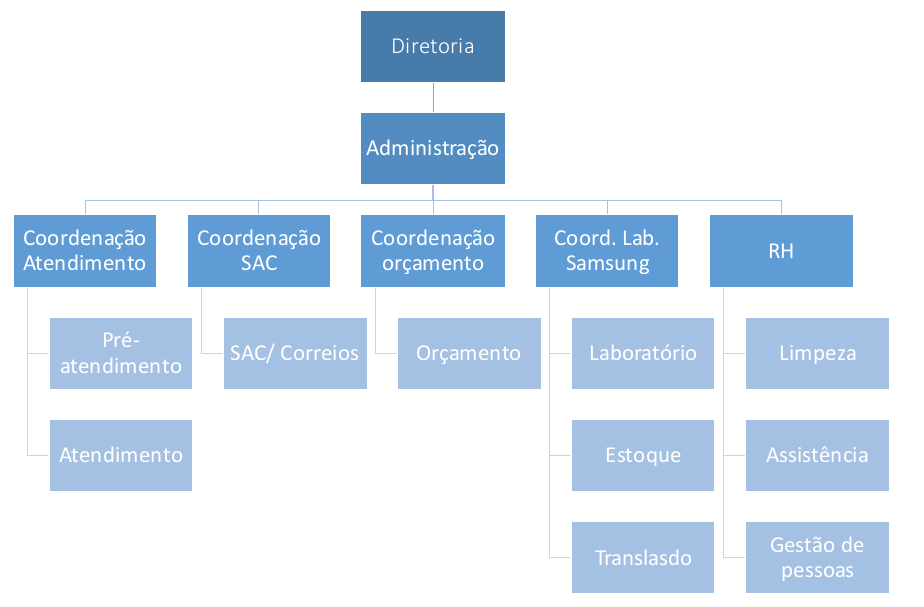
\includegraphics[width=0.5	\linewidth]{organograma_global.png} 
			
			\footnotesize{Fonte: Autor}
			\label{im1}
		\end{figure}	
	\end{frame}
	
	% SLIDE 4 - Fluxograma	
	\begin{frame}
		\frametitle{Fluxograma}
		\framesubtitle{Processos entre envio e recebimento do produto}
		
		\begin{minipage}[H]{.3\textwidth}
			\begin{itemize}
				\item \textit{Cliente};
				\item \textit{Atendimento/SAC};
				\item \textit{Translado};
				\item \textit{\textbf{Laboratório}};
				\item \textit{Estoque};
				\item \textit{\textbf{Laboratório}};
				\item \textit{\textbf{OQC}};
				\item \textit{SAC};
				\item \textit{Cliente};
			\end{itemize}
		\end{minipage}
		\hfill
		\begin{minipage}[H]{.65\textwidth}
			\begin{figure}
				\centering
				\caption{Fluxograma Global Express}
			
				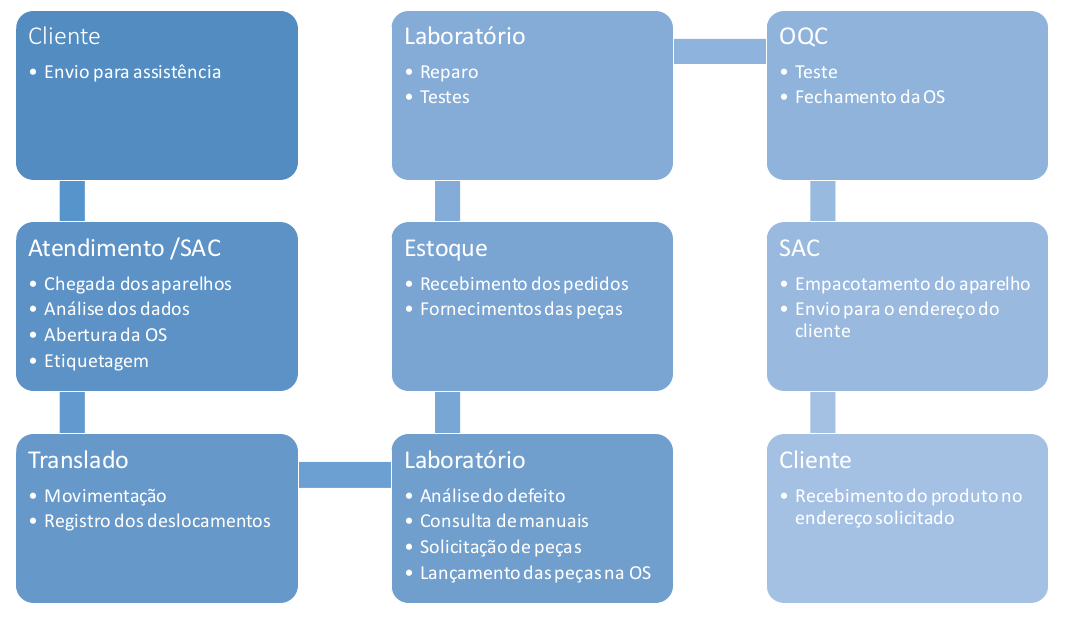
\includegraphics[width=0.8	\linewidth]{fluxograma_global.png} 
			
				\footnotesize{Fonte: Autor}
				\label{im1}
			\end{figure}
		\end{minipage}
	\end{frame}

%---------------------------------------------------------------------------
	% SEGUNDA SECAO
	\subsection{O estagiário}
%---------------------------------------------------------------------------
	% SLIDE 5 - Intodução Estagiário	
	\begin{frame}
		\frametitle{O estagiário}
		\framesubtitle{Como foi o estágio...}
		
		\begin{minipage}[H]{.3\textwidth}
			\begin{itemize}
				\item \textit{Apresentação da empresa};
				\begin{itemize}
					\item \textit{Espaços da empresa}
					\item \textit{Normas e regras}
					\item \textit{Segurança}
					\item \textit{Organização}
					\item \textit{Processo}
					\item \textit{Observação (1 mês)}
				\end{itemize}
			\end{itemize}
		\end{minipage}
		\hfill
		\begin{minipage}[H]{.3\textwidth}
			\begin{itemize}
				\item \textit{OQC};
				\begin{itemize}
					\item \textit{Auxílio}
					\item \textit{Meta}
					\item \textit{Produção}
					\item \textit{Trabalho Individual}
					\item \textit{Cobrança}
				\end{itemize}
			\end{itemize}
		\end{minipage}
		\hfill
		\begin{minipage}[H]{.3\textwidth}
			\begin{itemize}
				\item \textit{Laboratório};
				\begin{itemize}
					\item \textit{Auxílio}
					\item \textit{Segurança - ESD}
					\item \textit{Manutenção}
					\item \textit{Responsabilidade}
					\item \textit{Trabalho Individual}
					\item \textit{Cobrança*}
				\end{itemize}
			\end{itemize}
		\end{minipage}
	\end{frame}
	
	%---------------------------------------------------------------------------
	% SEGUNDA SECAO
	\section{SAMSUNG}
	\subsection{Monitoria}
%---------------------------------------------------------------------------
	% SLIDE 5 - Samsung	
	\begin{frame}
		\frametitle{SAMSUNG}
		\framesubtitle{Análise, Inspeção e Controle}
		
		\begin{minipage}[H]{.4\textwidth}
			\begin{itemize}
				\item \textit{GSPN};
				\begin{itemize}
					\item \textit{Controle}
					\item \textit{Qualidade}
					\item \textit{Serviços}
					\item \textit{Treinamentos}
				\end{itemize}
			\end{itemize}
		\end{minipage}
		\hfill
		\begin{minipage}[H]{.4\textwidth}
			\begin{itemize}
				\item \textit{Visitas Técnicas};
				\begin{itemize}
					\item \textit{Monitoramento}
					\item \textit{Pesquisa (motivos)}
					\item \textit{Inspeção}
					\item \textit{Análise de processo}
					\item \textit{Acompanhamento}
				\end{itemize}
			\end{itemize}
		\end{minipage}
		\hfill
		\begin{minipage}[H]{.4\textwidth}
			\begin{itemize}
				\item \textit{Fábrica};
				\begin{itemize}
					\item \textit{Recolhimento}
					\item \textit{Documentação}
					\item \textit{Dicas de Reparo}
					\item \textit{Defeitos de fabricação}
				\end{itemize}
			\end{itemize}
		\end{minipage}
	\end{frame}
	
%---------------------------------------------------------------------------
	%SECAO DE REFERENCIAS
	\section{Refer\^{e}ncias bibliogr\'{a}ficas}
%---------------------------------------------------------------------------
	% SLIDE 6 - REFERENCIAS
	\begin{frame}
		%[allowframebreaks]
		\frametitle{Refer\^{e}ncias bibliogr\'{a}ficas}
		\bibliography{Referencias}
	\end{frame}
	%---------------------------------------------------------------------------
\end{document}
